% ------------------------------------------------------------------------
% Relatorio da Entrega 2 -- Integracao iEducar x Moodle
% Baseado no "Modelo Canonico de Trabalho Academico com abnTeX2"
% (https://github.com/abntex/abntex2), enxugado para um relatorio tecnico
% de disciplina (sem ficha catalografica / folha de aprovacao / dedicatoria /
% epigrafe / resumos multilingues, que nao se aplicam aqui).
% ------------------------------------------------------------------------

\documentclass[
	12pt, openright, twoside, a4paper,
	english,
	brazil
	]{abntex2}

\usepackage{lmodern}
\usepackage[T1]{fontenc}
\usepackage[utf8]{inputenc}
\usepackage{lastpage}
\usepackage{indentfirst}
\usepackage{color}
\usepackage{graphicx}
\usepackage{microtype}
\usepackage{tikz}
\usepackage{listings}
\usetikzlibrary{arrows.meta, positioning, shapes.symbols, fit}

\usepackage[brazilian,hyperpageref]{backref}
\usepackage[alf]{abntex2cite}

\renewcommand{\backrefpagesname}{Citado na(s) p\'agina(s):~}
\renewcommand{\backref}{}
\renewcommand*{\backrefalt}[4]{
	\ifcase #1 %
		Nenhuma cita\c{c}\~ao no texto.%
	\or
		Citado na p\'agina #2.%
	\else
		Citado #1 vezes nas p\'aginas #2.%
	\fi}%

% ---
% Dados para CAPA e FOLHA DE ROSTO -- ajuste os campos entre [ ] antes de entregar
% ---
\titulo{Integra\c{c}\~ao entre iEducar e Moodle por meio de uma\\ Aplica\c{c}\~ao de Integra\c{c}\~ao Monol\'itica}
\autor{[NOME COMPLETO DO(S) INTEGRANTE(S) DO GRUPO]}
\local{Brasil}
\data{2026}
\orientador{[NOME DO(A) PROFESSOR(A)]}
\instituicao{%
  [NOME DA INSTITUI\c{C}\~AO]
  \par
  [NOME DO CURSO]
  \par
  Disciplina de Arquitetura de Software -- Entrega 2}
\tipotrabalho{Trabalho acad\^emico (Entrega 2)}
\preambulo{Relat\'orio t\'ecnico apresentado como Entrega 2 da disciplina de
Arquitetura de Software, descrevendo a implementa\c{c}\~ao de uma aplica\c{c}\~ao
de integra\c{c}\~ao entre os sistemas iEducar e Moodle.}

\definecolor{blue}{RGB}{41,5,195}
\makeatletter
\hypersetup{
		pdftitle={\@title},
		pdfauthor={\@author},
    	pdfsubject={\imprimirpreambulo},
	    pdfcreator={LaTeX with abnTeX2},
		pdfkeywords={ieducar}{moodle}{integracao}{arquitetura de software},
		colorlinks=true,
    	linkcolor=blue,
    	citecolor=blue,
		filecolor=magenta,
		urlcolor=blue,
		bookmarksdepth=4
}
\makeatother

\setlength{\parindent}{1.3cm}
\setlength{\parskip}{0.2cm}

\begin{document}

\frenchspacing

% ----------------------------------------------------------
% ELEMENTOS PRE-TEXTUAIS
% ----------------------------------------------------------

\imprimircapa
\imprimirfolhaderosto

% ---
% Resumo em portugues
% ---
\setlength{\absparsep}{18pt}
\begin{resumo}
Este trabalho apresenta a implementa\c{c}\~ao de uma aplica\c{c}\~ao de integra\c{c}\~ao entre o
iEducar, sistema de gest\~ao escolar, e o Moodle, ambiente virtual de aprendizagem, dando
continuidade ao planejamento arquitetural produzido na Entrega~1 da disciplina. A integra\c{c}\~ao
foi implementada como uma aplica\c{c}\~ao monol\'itica em Node.js/TypeScript, que consome
periodicamente a API REST j\'a existente do iEducar para ler turmas e matr\'iculas e, a partir
dela, cria e mant\'em cursos e inscri\c{c}\~oes correspondentes no Moodle por meio dos seus Web
Services REST. Os tr\^es componentes -- iEducar, Moodle e a aplica\c{c}\~ao de integra\c{c}\~ao --
s\~ao orquestrados por um \'unico ambiente Docker Compose. O trabalho descreve as decis\~oes de
arquitetura tomadas, os mecanismos de idempot\^encia e tratamento de falhas adotados, os testes
automatizados realizados e as limita\c{c}\~oes identificadas durante a implementa\c{c}\~ao.

\vspace{\onelineskip}

\noindent
\textbf{Palavras-chave}: integra\c{c}\~ao de sistemas. iEducar. Moodle. arquitetura monol\'itica. Docker.
\end{resumo}

% ---
% Abstract
% ---
\begin{resumo}[Abstract]
 \begin{otherlanguage*}{english}
This work presents the implementation of an integration application between iEducar, a school
management system, and Moodle, a learning management system, following up on the architectural
planning produced in the course's first deliverable. The integration was implemented as a
monolithic Node.js/TypeScript application that periodically polls iEducar's existing REST API to
read school classes and enrollments, creating and maintaining the corresponding Moodle courses and
enrolments through its REST web services. The three components -- iEducar, Moodle and the
integration application -- are orchestrated by a single Docker Compose environment. The report
describes the architectural decisions made, the idempotency and failure-handling mechanisms
adopted, the automated tests performed, and the limitations identified during implementation.

   \vspace{\onelineskip}

   \noindent
   \textbf{Key-words}: systems integration. iEducar. Moodle. monolithic architecture. Docker.
 \end{otherlanguage*}
\end{resumo}

\pdfbookmark[0]{\listfigurename}{lof}
\listoffigures*
\cleardoublepage

\pdfbookmark[0]{\listtablename}{lot}
\listoftables*
\cleardoublepage

\begin{siglas}
  \item[ABNT] Associa\c{c}\~ao Brasileira de Normas T\'ecnicas
  \item[API] Application Programming Interface
  \item[AVA] Ambiente Virtual de Aprendizagem
  \item[REST] Representational State Transfer
  \item[JSON] JavaScript Object Notation
  \item[SQL] Structured Query Language
  \item[ORM] Object-Relational Mapping
  \item[TS] TypeScript
\end{siglas}

\pdfbookmark[0]{\contentsname}{toc}
\tableofcontents*
\cleardoublepage

% ----------------------------------------------------------
% ELEMENTOS TEXTUAIS
% ----------------------------------------------------------
\textual

% ----------------------------------------------------------
\chapter{Introdu\c{c}\~ao e objetivo}
% ----------------------------------------------------------

Na Entrega~1 desta disciplina foi produzido o planejamento arquitetural de uma integra\c{c}\~ao
entre dois sistemas monol\'iticos legados: o \textbf{iEducar}, sistema de gest\~ao escolar
(matr\'iculas, turmas, servidores), e o \textbf{Moodle}, ambiente virtual de aprendizagem. Aquele
planejamento identificou quais informa\c{c}\~oes fariam sentido sincronizar, onde cada uma est\'a
armazenada no iEducar, quando a sincroniza\c{c}\~ao deveria ocorrer e quais mecanismos de cada
sistema poderiam ser usados como ponto de integra\c{c}\~ao.

O objetivo desta Entrega~2 \'e \textbf{implementar} esse planejamento: construir uma aplica\c{c}\~ao
de integra\c{c}\~ao real, como um terceiro componente monol\'itico entre os outros dois, capaz de
ler dados do iEducar e refleti-los no Moodle de forma correta, idempotente e tolerante a falhas,
executando tudo em um \'unico ambiente orquestrado por Docker Compose.

% ----------------------------------------------------------
\chapter{Informa\c{c}\~oes sincronizadas}
% ----------------------------------------------------------

Foram implementados os dois casos de integra\c{c}\~ao identificados na Entrega~1:

\begin{enumerate}
  \item \textbf{Turma (iEducar) \textrightarrow{} Curso (Moodle)}: cada turma ativa do ano letivo
  corrente, armazenada em \texttt{pmieducar.turma} (model \texttt{LegacySchoolClass} no c\'odigo do
  iEducar), gera um curso correspondente no Moodle.
  \item \textbf{Enturma\c{c}\~ao (iEducar) \textrightarrow{} Inscri\c{c}\~ao (Moodle)}: o v\'inculo
  entre um aluno e uma turma, armazenado em \texttt{pmieducar.matricula\_turma} (model
  \texttt{LegacyEnrollment}), gera a inscri\c{c}\~ao (\emph{enrolment}) do usu\'ario correspondente
  no curso do Moodle, com o papel de estudante.
\end{enumerate}

Ambos os dados s\~ao lidos pela API REST j\'a existente do iEducar
(\texttt{GET /api/school-class} e \texttt{GET /api/registration}), sem nenhuma altera\c{c}\~ao no
c\'odigo do monol\'ito do iEducar -- decis\~ao detalhada no Cap\'itulo~\ref{cap:decisoes}.

% ----------------------------------------------------------
\chapter{Arquitetura}
% ----------------------------------------------------------

A integra\c{c}\~ao \'e composta por tr\^es componentes, cada um um monol\'ito independente,
orquestrados por um \'unico Docker Compose na raiz do reposit\'orio (usando a diretiva
\texttt{include}, que permite reunir os \texttt{docker-compose.yml} j\'a existentes do iEducar e do
Moodle sem modific\'a-los~\cite{docker-compose-include}):

\begin{figure}[htb]
\centering
\caption{Vis\~ao geral da arquitetura e do fluxo de sincroniza\c{c}\~ao}
\label{fig:arquitetura}
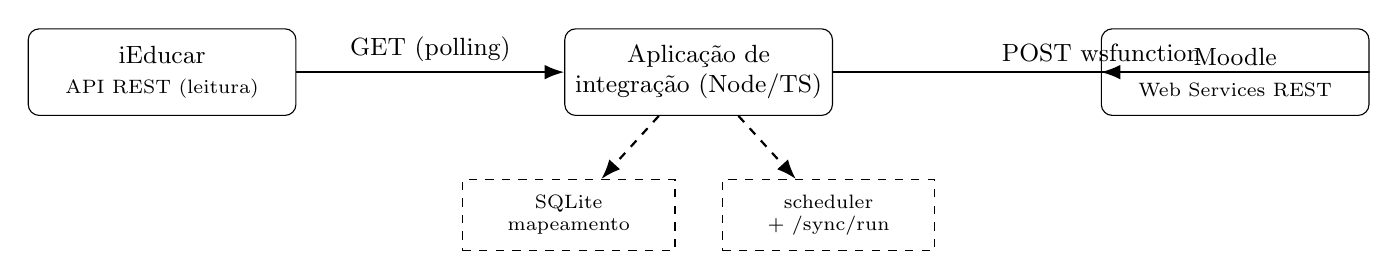
\begin{tikzpicture}[
  font=\small,
  box/.style={draw, rounded corners, minimum height=1.1cm, minimum width=3.4cm, align=center},
  sub/.style={draw, dashed, minimum height=0.9cm, minimum width=2.7cm, align=center, font=\scriptsize},
  arr/.style={-{Latex[length=2.5mm]}, thick}
]
  \node[box] (ieducar) {iEducar\\\scriptsize API REST (leitura)};
  \node[box, right=3.4cm of ieducar] (integra) {Aplica\c{c}\~ao de\\integra\c{c}\~ao (Node/TS)};
  \node[box, right=3.4cm of integra] (moodle) {Moodle\\\scriptsize Web Services REST};

  \node[sub, below=0.5cm of integra, xshift=-1.65cm, yshift=-0.3cm] (store) {SQLite\\mapeamento};
  \node[sub, below=0.5cm of integra, xshift=1.65cm, yshift=-0.3cm] (sched) {scheduler\\+ /sync/run};

  \draw[arr] (ieducar.east) -- node[above]{GET (polling)} (integra.west);
  \draw[arr] (integra.east) -- node[above]{POST wsfunction} (moodle.east |- integra.east) -- (moodle.west);
  \draw[arr, dashed] (integra) -- (store);
  \draw[arr, dashed] (integra) -- (sched);
\end{tikzpicture}
\end{figure}

\section{Compartimenta\c{c}\~ao interna da aplica\c{c}\~ao de integra\c{c}\~ao}

Internamente, a aplica\c{c}\~ao segue uma separa\c{c}\~ao inspirada em \emph{ports and adapters}:

\begin{itemize}
  \item \textbf{Adaptadores} (\texttt{src/adapters}): isolam o protocolo externo de cada sistema
  -- autentica\c{c}\~ao Bearer e pagina\c{c}\~ao do iEducar; formato de par\^ametros estilo PHP e
  convers\~ao de erros do protocolo REST do Moodle.
  \item \textbf{Dom\'inio} (\texttt{src/domain}): fun\c{c}\~oes puras de mapeamento (turma
  \textrightarrow{} curso, pessoa \textrightarrow{} usu\'ario), sem nenhuma chamada de rede --
  o que as torna test\'aveis isoladamente (Cap\'itulo~\ref{cap:testes}).
  \item \textbf{Orquestra\c{c}\~ao} (\texttt{src/sync}): combina os adaptadores e o dom\'inio,
  decide o que criar/atualizar, e isola falhas por item.
  \item \textbf{Persist\^encia} (\texttt{src/store}): SQLite local com as tabelas de mapeamento de
  IDs e o hist\'orico de execu\c{c}\~oes, base da idempot\^encia (Cap\'itulo~\ref{cap:decisoes}).
  \item \textbf{Entrada} (\texttt{src/scheduler.ts}, \texttt{src/server.ts}): disparam o ciclo de
  sincroniza\c{c}\~ao periodicamente ou sob demanda (\texttt{POST /sync/run}).
\end{itemize}

% ----------------------------------------------------------
\chapter{Decis\~oes t\'ecnicas}
\label{cap:decisoes}
% ----------------------------------------------------------

\section{Leitura por polling na API existente, em vez de evento novo no iEducar}

A Entrega~1 havia apontado o padr\~ao de evento~+~\emph{webhook} (usado pelo pr\'oprio iEducar na
integra\c{c}\~ao com o i-Di\'ario) como o caminho mais fiel para sincroniza\c{c}\~ao imediata.
Para esta entrega, optou-se por \textbf{consumir a API REST de leitura j\'a existente do iEducar}
(\texttt{GET /api/school-class}, \texttt{GET /api/registration}) via \emph{polling} peri\'odico,
em vez de alterar o c\'odigo do monol\'ito do iEducar. Essa decis\~ao reduz o risco de regress\~ao
em um sistema de terceiros e mant\'em a aplica\c{c}\~ao de integra\c{c}\~ao como o \'unico lugar
onde a l\'ogica de sincroniza\c{c}\~ao vive -- ao custo de n\~ao reagir instantaneamente a
mudan\c{c}as (mitigado pelo intervalo configur\'avel e pelo disparo manual).

\section{Autentica\c{c}\~ao}

A API do iEducar n\~ao expõe nenhum endpoint HTTP de login; o token (Laravel Sanctum, sem
expira\c{c}\~ao) \'e gerado uma vez via linha de comando
(\texttt{php artisan admin:token}, comando j\'a existente no projeto) e configurado na
aplica\c{c}\~ao de integra\c{c}\~ao~\cite{laravel-sanctum}. No Moodle, o token do Web Service REST
\'e gerado pela interface administrativa, associado a um servi\c{c}o externo restrito \`as
fun\c{c}\~oes estritamente necess\'arias~\cite{moodle-ws-docs}.

\section{Idempot\^encia e consist\^encia}

Cada turma e cada enturma\c{c}\~ao processada \'e registrada numa tabela SQLite pr\'opria da
aplica\c{c}\~ao de integra\c{c}\~ao, relacionando o identificador do iEducar ao identificador
correspondente no Moodle. Antes de criar um curso ou inscrever um usu\'ario, a aplica\c{c}\~ao
sempre consulta esse mapeamento; como rede de seguran\c{c}a adicional (por exemplo, se o banco
local for perdido), tamb\'em consulta o pr\'oprio Moodle por \texttt{shortname}/\texttt{idnumber}
determin\'isticos antes de criar qualquer recurso, evitando duplica\c{c}\~ao mesmo em reexecu\c{c}\~oes.

\section{Tratamento de falhas}

A falha ao sincronizar uma turma ou uma enturma\c{c}\~ao espec\'ifica \'e isolada e registrada
(com o contexto do item e a mensagem de erro) sem interromper o processamento das demais -- uma
turma com dado inconsistente, por exemplo, n\~ao impede que as outras sejam sincronizadas no mesmo
ciclo. Cada execu\c{c}\~ao do ciclo de sincroniza\c{c}\~ao \'e registrada com contadores e a lista
de erros, consult\'avel via \texttt{GET /sync/status}.

\section{Limita\c{c}\~ao de dados de identidade}
\label{sec:limitacao-identidade}

Os endpoints de leitura usados n\~ao expõem diretamente nome e e-mail do aluno junto da
enturma\c{c}\~ao; a resolu\c{c}\~ao completa dessa identidade (necess\'aria para criar um usu\'ario
do Moodle com dados reais, em vez de um nome provis\'orio derivado do identificador) \'e discutida
como limita\c{c}\~ao no Cap\'itulo~\ref{cap:limitacoes}.

% ----------------------------------------------------------
\chapter{Testes realizados}
\label{cap:testes}
% ----------------------------------------------------------

Por se tratar de uma integra\c{c}\~ao entre sistemas externos, a estrat\'egia de testes priorizou
\textbf{testes unit\'arios da camada de dom\'inio e de orquestra\c{c}\~ao}, com os adaptadores de
rede substitu\'idos por \emph{mocks} -- sem depend\^encia de iEducar/Moodle realmente no ar durante
a execu\c{c}\~ao da su\'ite. Os testes cobrem, entre outros casos:

\begin{itemize}
  \item mapeamento correto dos campos crus da API do iEducar para o modelo normalizado;
  \item gera\c{c}\~ao determin\'istica de \texttt{shortname}/\texttt{idnumber} do curso no Moodle;
  \item \textbf{idempot\^encia}: uma segunda execu\c{c}\~ao do ciclo sobre os mesmos dados n\~ao
  cria curso/inscri\c{c}\~ao duplicados;
  \item atualiza\c{c}\~ao do curso no Moodle quando o nome da turma muda no iEducar, sem duplicar;
  \item \textbf{isolamento de falhas}: quando a cria\c{c}\~ao de um curso falha, as demais turmas
  do mesmo ciclo continuam sendo processadas;
  \item reaproveitamento de um usu\'ario j\'a existente no Moodle (por \texttt{idnumber}) em vez de
  criar um duplicado.
\end{itemize}

% ----------------------------------------------------------
\chapter{Resultados}
% ----------------------------------------------------------

% TODO: esta secao sera finalizada com a execucao real contra o ambiente Docker
% (contagens de /sync/status, curso de exemplo criado no Moodle, etc.)

% ----------------------------------------------------------
\chapter{Limita\c{c}\~oes}
\label{cap:limitacoes}
% ----------------------------------------------------------

\begin{itemize}
  \item \textbf{Identidade do aluno incompleta} (ver Se\c{c}\~ao~\ref{sec:limitacao-identidade}):
  usu\'arios do Moodle podem ser criados com nome provis\'orio quando a API do iEducar n\~ao
  disponibiliza nome/e-mail junto da enturma\c{c}\~ao consultada.
  \item \textbf{Senha inicial fixa e determin\'istica} para usu\'arios criados no Moodle -- adequado
  para demonstra\c{c}\~ao, mas inadequado para produ\c{c}\~ao, onde um fluxo de SSO/LTI seria
  necess\'ario.
  \item \textbf{Categoria \'unica no Moodle} para todos os cursos criados, configurada globalmente
  -- n\~ao h\'a, nesta vers\~ao, mapeamento de categoria por escola/s\'erie.
  \item \textbf{Consist\^encia eventual}: por depender de \emph{polling}, uma mudan\c{c}a no
  iEducar só se reflete no Moodle no pr\'oximo ciclo (ou quando disparada manualmente), nunca
  instantaneamente.
  \item \textbf{Papel de professor n\~ao implementado nesta entrega}: a infraestrutura de
  mapeamento de papel (\texttt{MOODLE\_ROLE}) j\'a suporta professor, mas a sincroniza\c{c}\~ao de
  \texttt{professor\_turma} n\~ao foi conectada por restri\c{c}\~ao de tempo.
\end{itemize}

% ----------------------------------------------------------
\chapter*{Conclus\~ao}
\addcontentsline{toc}{chapter}{Conclus\~ao}
% ----------------------------------------------------------

A implementa\c{c}\~ao confirmou que \'e poss\'ivel integrar dois monólitos legados sem alterar o
c\'odigo de nenhum dos dois, concentrando toda a l\'ogica de tradu\c{c}\~ao e sincroniza\c{c}\~ao
em um terceiro componente dedicado. O principal aprendizado t\'ecnico foi que a viabilidade dessa
abordagem depende diretamente da \textbf{riqueza da API de leitura j\'a exposta} pelo sistema de
origem -- quando ela n\~ao cobre totalmente o dado necess\'ario (caso da identidade do aluno,
Se\c{c}\~ao~\ref{sec:limitacao-identidade}), a aplica\c{c}\~ao de integra\c{c}\~ao precisa absorver
essa limita\c{c}\~ao ou, numa itera\c{c}\~ao futura, justificar uma pequena extens\~ao do sistema de
origem -- um trade-off cl\'assico de estrat\'egias de moderniza\c{c}\~ao incremental de
legados~\cite{fowler-strangler}.

% ----------------------------------------------------------------------
\postextual
% ----------------------------------------------------------------------

\bibliography{referencias}

\begin{apendicesenv}
\partapendices

% ----------------------------------------------------------
\chapter{Exemplo de chamada ao endpoint de status}
% ----------------------------------------------------------

\begin{lstlisting}[basicstyle=\small\ttfamily, breaklines=true]
curl -X POST http://localhost:3000/sync/run
curl http://localhost:3000/sync/status
\end{lstlisting}

\end{apendicesenv}

\end{document}
